\section{Implementação}
Nesta seção serão definidas as minucias que permeiam nossa aplicação, a qual foi implementada utilizando a linguagem de programação Python na versão estável 3.10.8 para as interfaces gráficas e interativas e para administrar nosso banco de dados foi empregado o SGBD (Sistema de Gerenciamento de Banco de Dados) foi utilizado o PostgreSQL, a integração e composição entre ambos foi feita utilizando o Docker e o driver Psycopg.

A aplicação consiste de um ambiente interativo que permite a realização de consultas pré-especificadas que serão expostas em maiores detalhes, e a realização de consultas personalizadas de acordo com a necessidade do usuário, dentre queries pré-estabelecidas. A interface de usuário foi feita baseada na biblioteca CustomTkinter, externa a linguagem de programação Python.
\subsection{Script de Consultas}

Os dados utilizados para as consultas (esquema, dados e consultas) pode ser encontrado no repositório da implementação, na pasta "data", \href{https://github.com/Franreno/AuxilioDepQuim/tree/main/data}{neste link}.


\lstset{language=SQL,
             basicstyle=\footnotesize,
             numbers=left,
             numberstyle=\footnotesize,
             frame=shadowbox,
             rulesepcolor=\color{red}}
\begin{itemize}
    \item \textbf{C1-Consultar informações do auxiliado referentes a sua reabilitação}
    
    \begin{lstlisting}
        SELECT A.NOME,C.NOME,R.PRESENCA 
        FROM REABILITACAO R 
        JOIN AUXILIADO A 
        ON R.DEPENDENTE = A.CPF 
        JOIN CLINICA C 
        ON R.CLINICA = C.CNPJ 
        WHERE(SELECT AVG(R1.PRESENCA) FROM REABILITACAO R1) < R.PRESENCA;  
    \end{lstlisting}
    
    Nesta consulta foi realizado o \textit{inner join} das tabelas REABILITACAO, AUXILIADO e CLINICA, a fim de extrair de cada uma delas o nome do AUXILIADO, a CLINICA que ele está em REABILITACAO e sua presença. A junção é realizada garantindo que só serão expostos auxiliados cujo a presença seja maior que a média geral de todos os auxiliados, isso é garantido pelas cláusulas ON presentes na consulta, que garantem a junção apenas de tuplas que atendam aos requisitos da cláusula WHERE.

    \item \textbf{C2-Consulta de empresas parceiras com vagas de emprego supervisionado}

    \begin{lstlisting}
        SELECT T.NOME, EP.NUFUNCIONARIOS, ES.LOCAL
        FROM TERCEIROS T
        JOIN EMPREGO_SUPERVISIONADO ES
        ON T.NUCPFCNPJ = ES.EMPRESA_PARCEIRA
        JOIN EMPRESAS_PARCEIRAS EP
        ON ES.EMPRESA_PARCEIRA = EP.CNPJ
        WHERE EP.MAXFUNCIONARIOS > EP.NUFUNCIONARIOS;
    \end{lstlisting}

    Neste procedimento são selecionados nome, número de funcionários trabalhando atualmente e local da vaga oferecida referentes a uma empresa parceira, estas informações estão presentes, respectivamente, nas tabelas TERCEIROS, EMPRESAS\_PARCEIRAS E EMPREGO\_SUPERVISIONADO. Como as informações que buscamos estão em tabelas distintas é utilizada a junção interna, representada em SQL pela cláusula JOIN, a garantia de coerência e objetividade das informações buscadas são garantidas pelas cláusulas ON, a qual realiza a junção apenas das tuplas que atendem as demandas feitas em WHERE e propaga isso de forma encadeada. A clausula WHERE garante que as tuplas selecionadas em EMPRESAS\_PARCEIRAS tenham um número máximo de funcionários maior que o número que já ocupa as vagas, i.e, pode receber novos trabalhadores.

    \item \textbf{C3-Consulta do status empregatício de um auxiliado} 
    
    \begin{lstlisting}
        SELECT A.NOME,
        CASE 
            WHEN  ES.DURACAO - CURRENT_DATE < 10 
            AND ES.DURACAO - CURRENT_DATE > 0
                THEN 'PROXIMO AO FIM'
            WHEN ES.DURACAO- CURRENT_DATE > 10 
                THEN 'FUNCIONARIO EMPREGADO'
            WHEN (ES.DURACAO - CURRENT_DATE < 0) 
            OR ES.DURACAO IS NULL
                THEN 'FUNCIONARIO DESEMPREGADO'
            END STATUS_EMPREGO
        FROM AUXILIADO A
        LEFT JOIN EMPREGO_SUPERVISIONADO ES
        ON A.CPF = ES.AUXILIADO
        LEFT JOIN TERCEIROS E
        ON ES.EMPRESA_PARCEIRA = E.NUCPFCNPJ;
    \end{lstlisting}

    Nesta consulta são retornadas tuplas com o nome do auxiliado associado ao seu status empregatício, baseado em uma subtração entre a duração do emprego supervisionado e a data atual. Isso foi feito através da cláusula CASE que pode classificar através da diretiva WHEN. Na aplicação, se o auxiliado tem menos de dez dias de emprego supervisionado planejados, é considerado que seu trabalho está PROXIMO AO FIM, caso contrário ele tem o status de FUNCIONARIO EMPREGADO caso tenha mais de dez dias até o fim de seu contrato ou está desempregado caso o atributo DURACAO seja nulo ou apresente uma data menor que a data atual.

    \item \textbf{C4-Consulta de todos os auxiliados empregados}

    \begin{lstlisting}
        SELECT * from AUXILIADO A
        JOIN EMPREGO_SUPERVISIONADO ES
        ON A.CPF = ES.AUXILIADO;
    \end{lstlisting}

    Nesta consulta nos interessa recuperar todas as tuplas de auxiliados que estão relacionadas a um emprego supervisionado, i.e, nos interessa saber quais auxiliados estão empregados e suas informações. O retorno apenas das tuplas da tabela AUXILIADO referentes a participantes com emprego ativo é garantido pela junção interna, representada pela cláusula JOIN em conjunto com a clásula ON, a qual delimita as tuplas de acordo com a condição apresentada. 

    \item \textbf{C5-Consulta de centros e de quantos auxiliados se beneficiam de sua tesouraria}

    \begin{lstlisting}
        SELECT C.NOME, COUNT(*) FROM
        CENTRO C JOIN TESOURARIA T
        ON C.CNPJ = T.CENTRO
        JOIN AUXILIADO A  
        ON A.FRENTE = T.FRENTE AND  T.CENTRO = A.CENTRO
        GROUP BY C.NOME;
    \end{lstlisting}

    Nesta consulta são retornadas as tuplas contendo os nomes de todos os centro que possuem tesouraria e quantos auxiliados são subsidiados pelas suas respectivas tesourarias. Nesta consulta foi utilizada a cláusula GROUP BY para realizar a contagem da quantidade de tuplas referente a grupos separados pelo nome dos centros selecionados. Além disso, as cláusulas JOIN associadas as cláusulas ON garantem que são selecionados apenas centros com tesourarias na primeira afirmação lógica, destas são segregadas apenas as tesourarias que possuem auxiliados na segunda afirmação lógica, por fim os centros comunitários são agrupados pelos seus respectivos nomes.

    \item \textbf{C6-Consulta os auxiliados que são apenas moradores de rua}

    \begin{lstlisting}
        SELECT A.NOME, A.LOCAL FROM
        AUXILIADO A JOIN TIPO_AUXILIADO TA
        ON A.CPF = TA.CPF
        WHERE A.CPF NOT IN
        (SELECT DISTINCT A.CPF FROM 
            AUXILIADO A JOIN TIPO_AUXILIADO TA
            ON A.CPF = TA.CPF
            WHERE UPPER(TA.TIPO) = 'DEPENDENTE_QUIMICO');
    \end{lstlisting}

    Nesta seleção são retornadas tuplas com nome e local dos auxiliados que são, exclusivamente, moradores de rua. A exclusividade do tipo de auxiliado vem da cláusula WHERE acompanhada de NOT IN, que não inclui os auxiliados cujo tipo é DEPENDENTE\_QUIMICO, a cláusula DISTINCT apenas evita repetições de tuplas selecionadas pela cláusula WHERE e garante otimização.
    
\end{itemize}
\subsection{Aplicação}

O repositório da aplicação pode ser encontrado \href{https://github.com/Franreno/AuxilioDepQuim}{neste link}.

\subsubsection{Requisitos do Sistema}
Além da linguagem de programação Python devidamente instalada em versão 3.8.2 ou maior é necessário instalar as dependências e o \textit{package manager} Pip referente a esta versão.

Todas as considerações feitas a seguir consideram que o usuário está utilizando um sistema operacional do tipo Linux baseado em Debian.

Para facilitar o uso da aplicação foram criados \textit{scripts} para instalação de algumas dependências, portanto é necessário estar no diretório raiz do projeto e permitir que os \textit{scripts} sejam executados através do seguinte comando no terminal:

\lstset{language=bash,
             basicstyle=\footnotesize,
             numbers=none,
             frame=shadowbox,
             rulesepcolor=\color{red}}

\begin{lstlisting}
    sudo chmod +x scripts/*.sh
\end{lstlisting}

Os pacotes Tkinter utilizado para construção da interface gráfica e Psycopg2 para integração com o PostreSQL tem como dependências os pacotes python-tk e libpq-dev respectivamente, para baixa-los basta utilizar o seguinte comando em sua shell:

\begin{lstlisting}
    sudo apt install python-tk libpq-dev
\end{lstlisting}

Para finalizar os pacotes basta baixa-los utilizando o administrador de pacotes nativo do Python, o pip, através de um arquivo de texto criado por comodidade e facilidade de uso:

\begin{lstlisting}
    pip install -r requirements.txt
\end{lstlisting}

Por fim, para realizar a instalação e a inicialização do Docker, ambiente de integração entre Python e o SGBD utilizado, basta realizar o seguinte comando em sua própria shell:

\begin{lstlisting}
    sudo scripts/install_docker_ubuntu.sh && sudo scripts/install.sh
\end{lstlisting}
\subsubsection{Funcionamento geral}
A fim de executar o programa basta utilizar o seguinte comando:

\begin{lstlisting}
    python src/main.py
\end{lstlisting}

Com isso, será exibida a interface vista na Figura \ref{fig:interface}, nela são perceptíveis os botões responsivos ao clique a esquerda, os quais desempenham as seguintes funções:
\begin{itemize}
    \item \textbf{Mostrar tabela}: É exibido um botão no estilo \textit{dropdown} contendo como opções todas as tabelas implementadas, ao selecionar uma tabela específica, são exibidas sua colunas, o tipo de cada uma e seu respectivo tamanho. É possível ver um exemplo da interface na Figura \ref{fig:mostratab}.
    \item \textbf{Rodar/Debugar SQL}: Permite a inserção direta de queries SQL através de uma interface de escrita, esta função está implementada única e exclusivamente para facilitar testes e correções e não estaria disponível ao usuário final. Funciona basicamente como um SQL injection liberado e implementado pelo sistema. Sua execução está referenciada pela Figura \ref{fig:rodarsql}, onde é possível ver uma janela inferior interativa, a qual recebe as queries, e uma janela superior, responsável por exibir os resultados.
    \item \textbf{Rodar consultas.sql}: Realiza as consultas previstas no arquivo pré-estabelecido pelos desenvolvedores. Sua execução está exposta na Figura\ref{fig:consultassql}, que exibe uma janela superior para o resultado das consultas.
    \item \textbf{Cadastrar novo funcionário, cadastrar empresa e inserir centro}: São funcionalidades de inserção de tuplas e possuem interfaces semelhantes, nessas são exibidos os atributos de cada tabela referenciada(Funcionário, Empresa Parceira e Centro Comunitário), os quais possuem um pequeno espaço para serem preenchidos os valores e um botão para confirmar a inserção. A interface referente a Cadastrar novo funcionário, que serve como base para as demais, está explicitada na Figura \ref{fig:novofunc}.
    \item \textbf{Mostrar informações}: É exibido um botão no estilo \textit{dropdown} com todas as tabelas possíveis e disponíveis para consulta, ao selecionar uma tabela é exibido um segundo botão \textit{dropdown} contendo todos os atributos da tabela, assim é possível conferir, por exemplo, todos os nomes dos auxiliados inseridos. A interface de uso pode ser vista na Figura \ref{fig:mostrarInfo}, já com os dois botões \textit{dropdown} exibidos.
\end{itemize}

Vale ressaltar que nas funcionalidades de inserção as strings inseridas nos campos delimitados são passadas como parâmetros de funções secundárias e não uma simples concatenação de strings, evitando ataques maliciosos.

\begin{figure}[H]
    \centering
    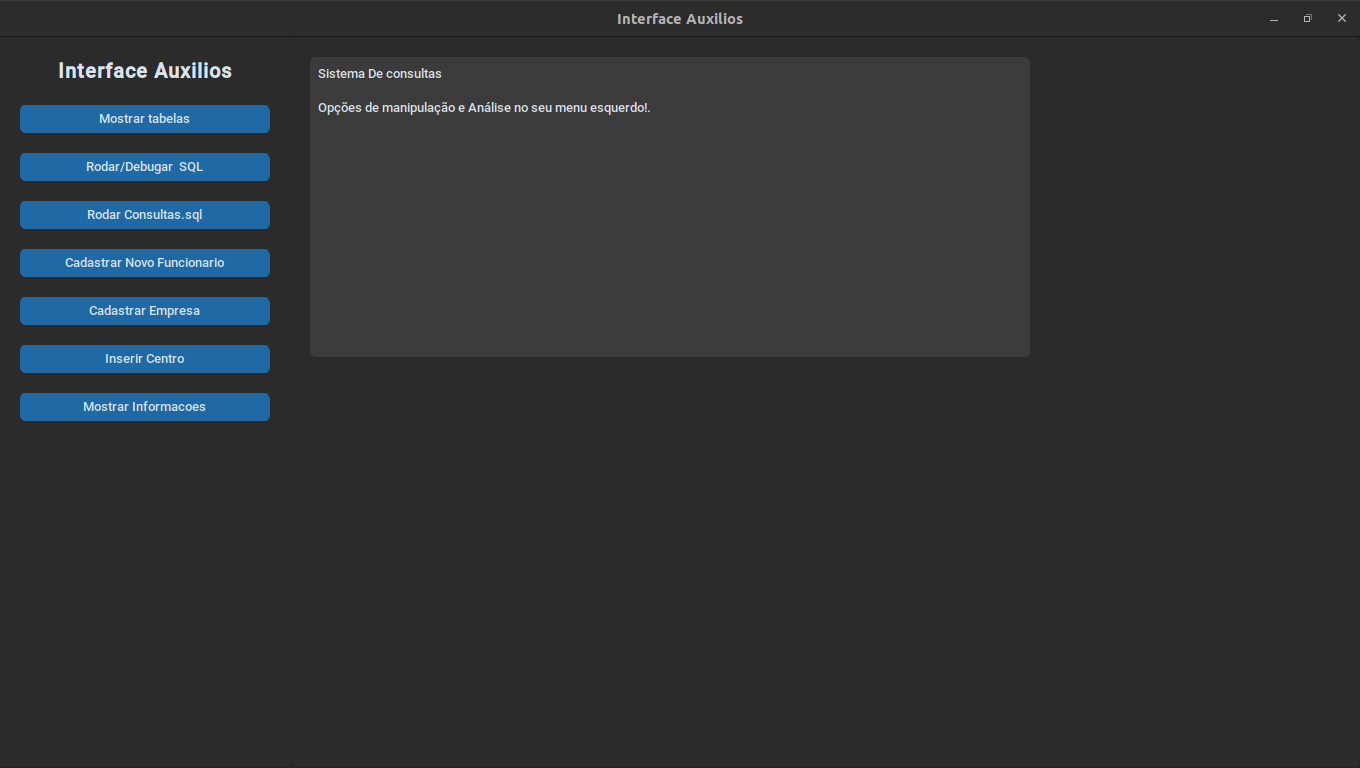
\includegraphics[scale=0.3]{images/interface.png}
    \caption{Interface inicial. \textbf{Fonte:} Autores}
    \label{fig:interface}
\end{figure}

\begin{figure}[H]
    \centering
    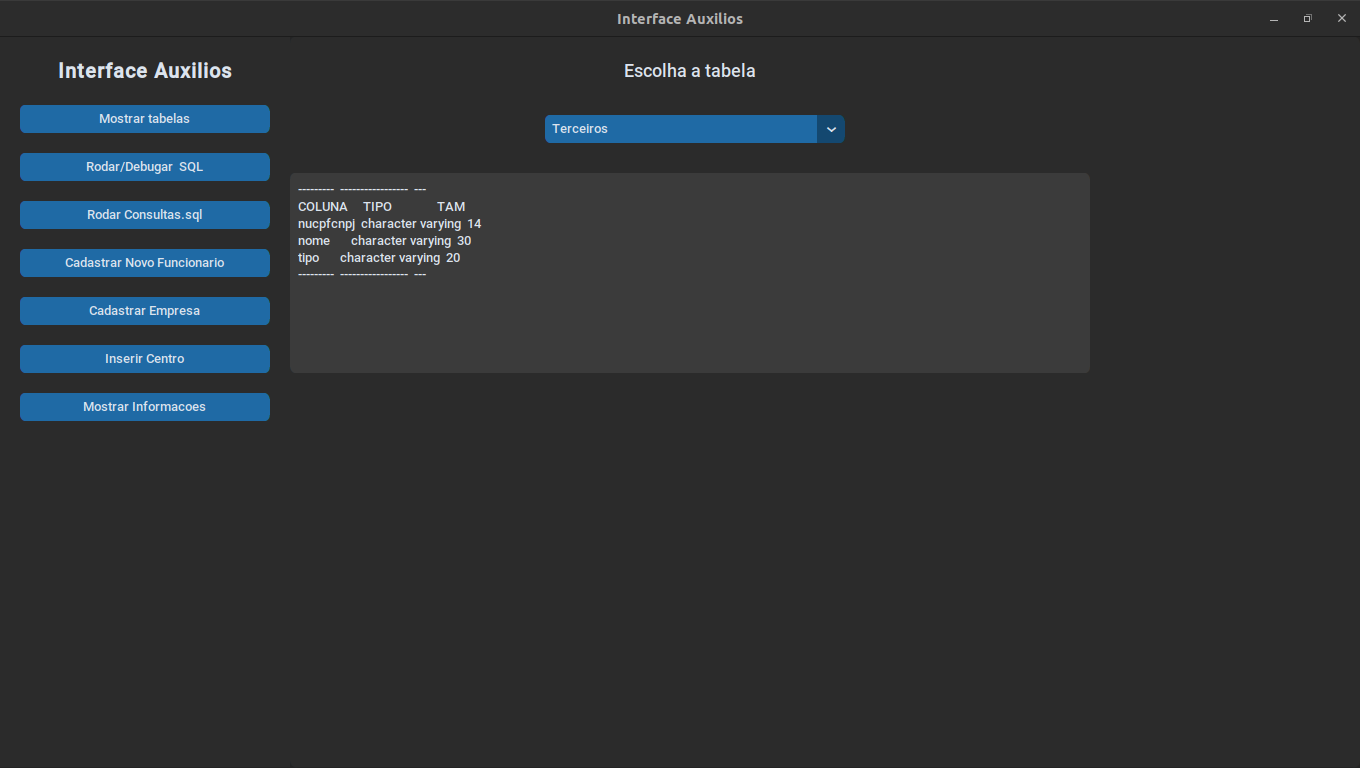
\includegraphics[scale=0.3]{images/mostratab.png}
    \caption{Interface ao selecionar o botão Mostrar tabela. \textbf{Fonte:} Autores}
    \label{fig:mostratab}
\end{figure}

\begin{figure}[H]
    \centering
    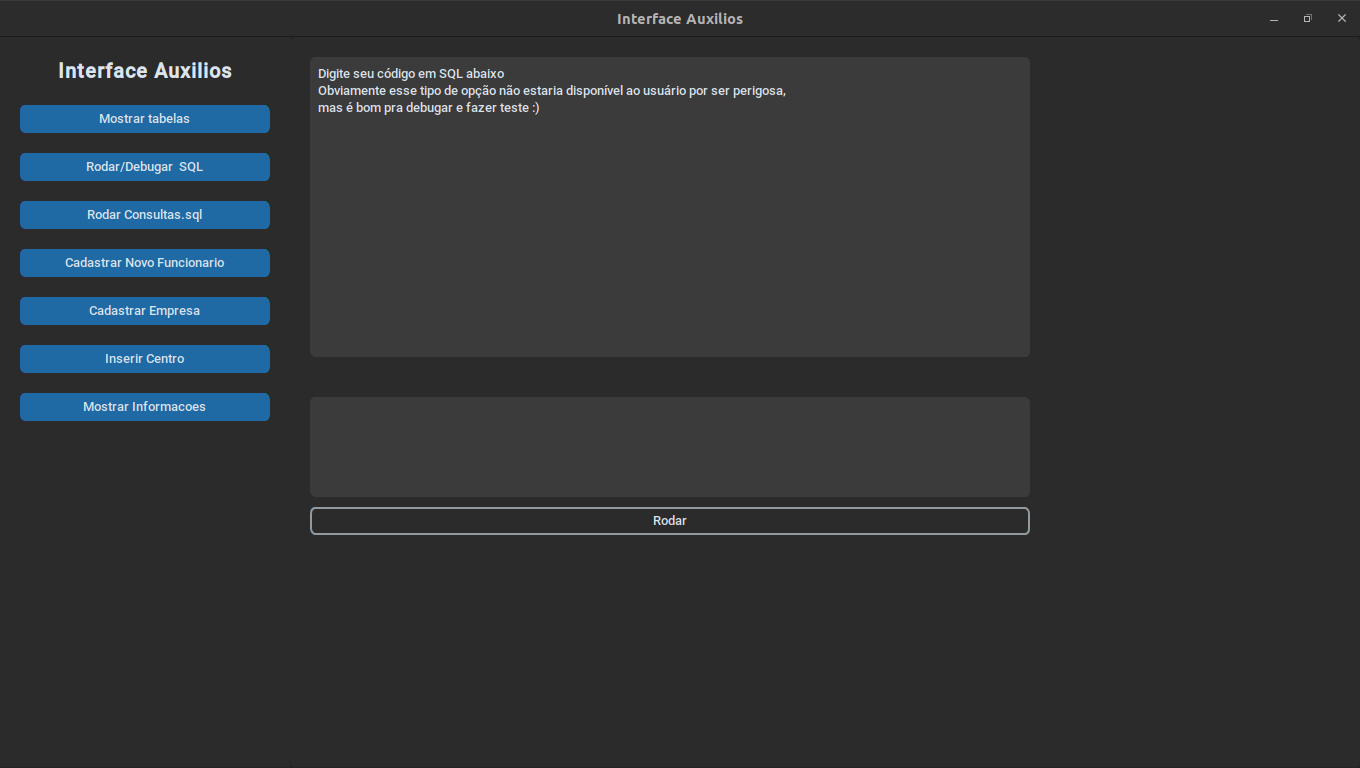
\includegraphics[scale=0.3]{images/rodarsql.png}
    \caption{Interface ao selecionar o botão Rodar/Debugar SQL. \textbf{Fonte:} Autores}
    \label{fig:rodarsql}
\end{figure}

\begin{figure}[H]
    \centering
    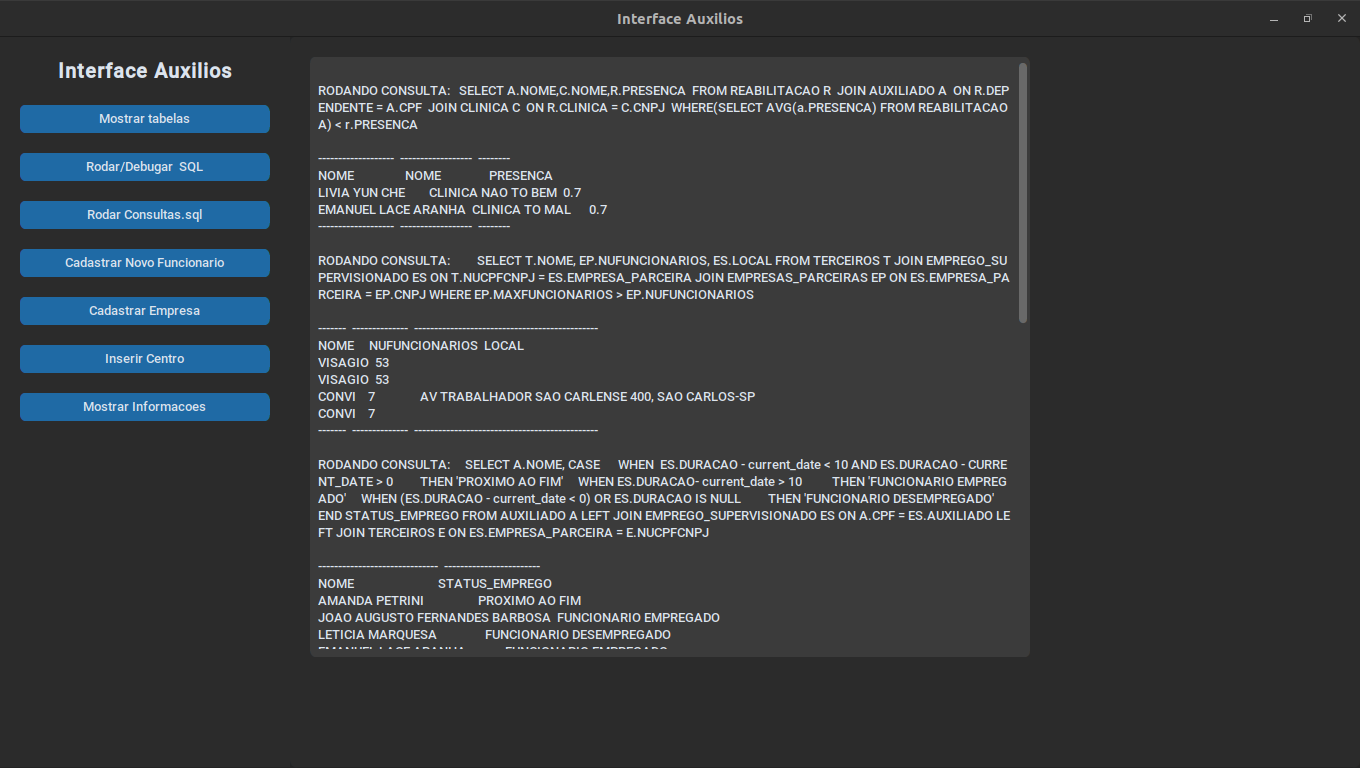
\includegraphics[scale=0.3]{images/consultassql.png}
    \caption{Interface ao selecionar o botão Rodar consultas.sql. \textbf{Fonte:} Autores}
    \label{fig:consultassql}
\end{figure}

\begin{figure}[H]
    \centering
    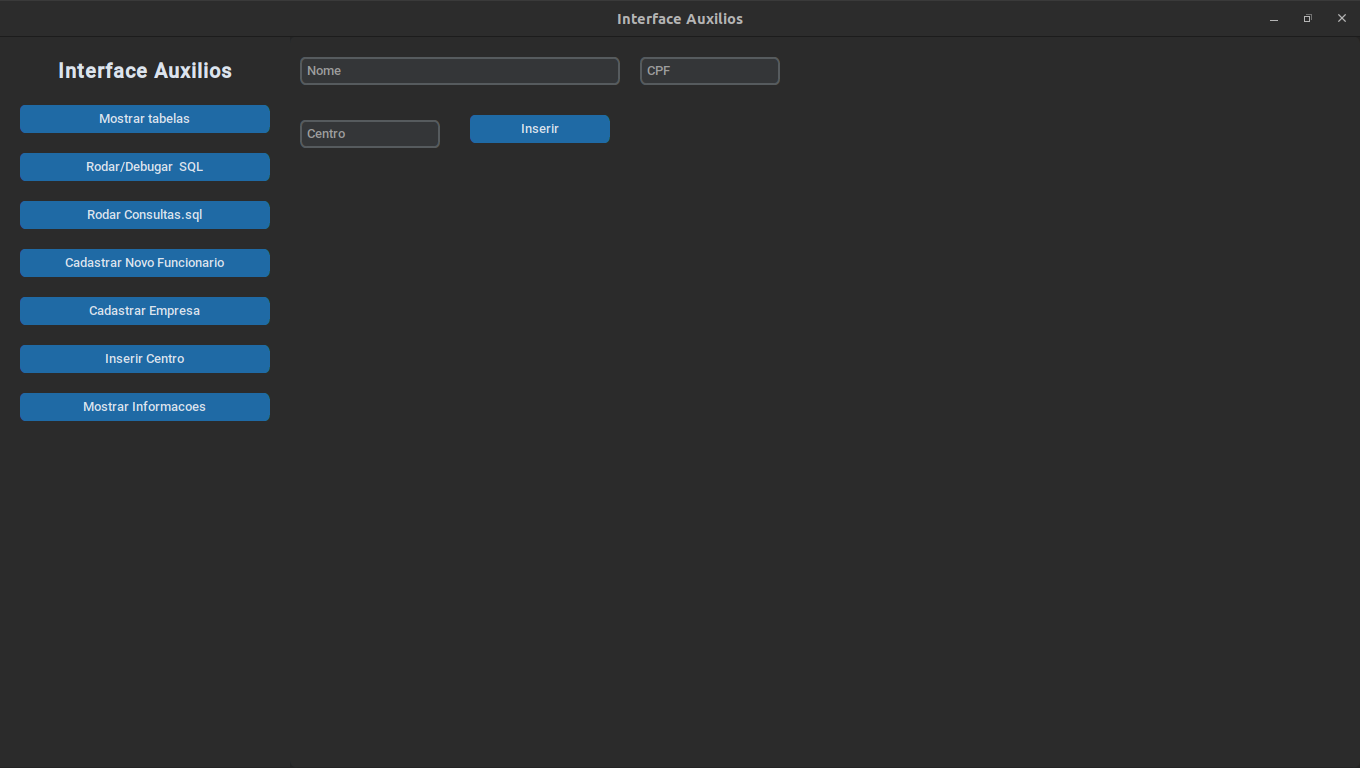
\includegraphics[scale=0.3]{images/novofunc.png}
    \caption{Interface ao selecionar o botão Cadastrar novo funcionário. \textbf{Fonte:} Autores}
    \label{fig:novofunc}
\end{figure}

\begin{figure}[H]
    \centering
    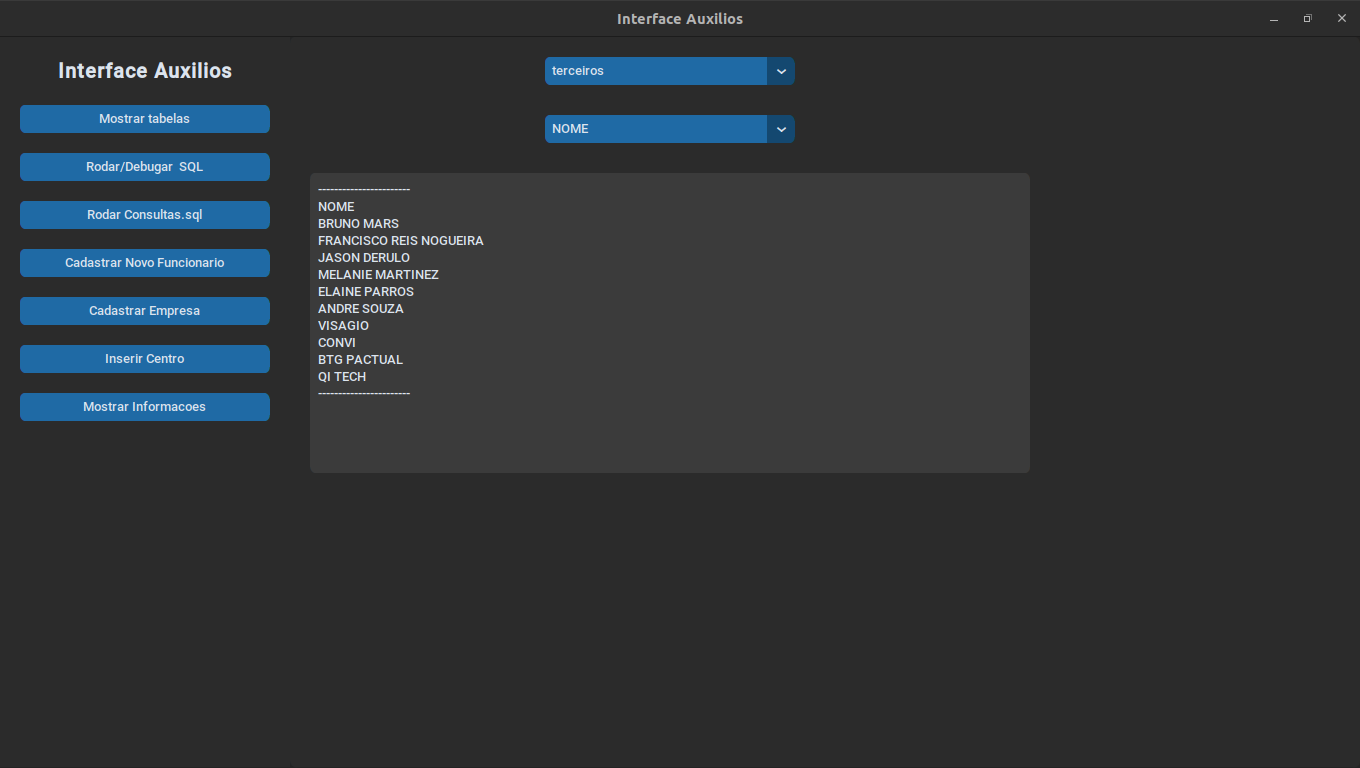
\includegraphics[scale=0.3]{images/mostrarInfo.png}
    \caption{Interface ao selecionar o botão Mostrar informações. \textbf{Fonte:} Autores}
    \label{fig:mostrarInfo}
\end{figure}

